\section{Anhang}


\subsection{Substitution bei Integralen}
% Von Zusammenfassung Analysis 2a

\begin{tabular}{ll}
    $\int \limits_0^{\sqrt{\pi}} x^3 \cdot \cos(x^2) \, \diff x$    & \cbl{Substitution: $a = x^2$ } \crd{ \textbf{auch auf Grenzen anwenden!}}                                                 \\
                                                                    & \cbl{$\diff a = 2 \, x \cdot \, \diff x$ \textrightarrow\ $\diff x = \frac{\diff a}{2x} = \frac{\diff a}{2 \sqrt{a}}$}
\end{tabular}

$\int \limits_{\crd{0}}^{\crd{\pi}} a \, \sqrt{a} \cdot \cos(a) \frac{\diff a}{2 \sqrt{a}} 
    = \int \limits_{\crd{0}}^{\crd{\pi}} a \, \sqrt{a} \cdot \cos(a) \, \frac{1}{2} \frac{1}{\sqrt{a}} \, \diff a
    = \frac{1}{2} \int \limits_{\crd{0}}^{\crd{\pi}} a \cdot \cos(a) \, \diff a = \ldots $


\subsubsection{Partielle Integration (Produktregel)}
\vspace{-1em}

\[\int_{a}^{b} f'\cdot g \, \diff x = \left[ f\cdot g \right]_{a}^{b} - \int_{a}^{b} f\cdot g' \, \diff x
\quad \text{oder} \quad
\int_{a}^{b} f\cdot g' \, \diff x = \left[ f\cdot g \right]_{a}^{b} - \int_{a}^{b} f' \cdot g \, \diff x
\]

Partielle Integration darf mehrfach angewendet werden. \\
\textbf{PI sollte wenn möglich vermieden werden! Produkte in Summen umschreiben!}\vspace{1em}

\textbf{LIATE} - Priorität für $g$ - funzione da derivare (non $\dots'$ nella forma base):


\subsection{Wichtige Integrale}

\begin{minipage}{0.48\columnwidth}
    $$ \frac{1}{T} \int\limits_{-T/2}^{T/2} \sin^2(\omega \, t) \,\diff t = \frac{1}{2} $$
\end{minipage}
\hfill
\begin{minipage}{0.48\columnwidth}
    $$ \frac{1}{T} \int\limits_{-T/2}^{T/2} \cos^2(\omega \, t) \, \diff t = \frac{1}{2} $$
\end{minipage}


\subsection{Trigonometrie}


% von Integraltransformationen Zusammenfassung	 
% \includegraphics[width=\columnwidth]{images/trigo.png} 

\begingroup
\renewcommand{\arraystretch}{2}
\setlength{\tabcolsep}{0mm}
\scalebox{0.33}{
\Huge
\begin{tabularx}{3\columnwidth}{rp{1mm}V{3}*{17}{C}}
    \rowcolor{subsectioncolor!30}$\bm{\alpha}$\phantom{${}^{\circ}$} && $0$ & $\dfrac{\pi}{6\mathstrut}$ & $\dfrac{\pi}{4}$ & $\dfrac{\pi}{3}$ & $\dfrac{\pi}{2}$ & $\dfrac{2\pi}{3}$ & $\dfrac{3\pi}{4}$ & $\dfrac{5\pi}{6}$ & $\pi$ & $\dfrac{7\pi}{6}$ & $\dfrac{5\pi}{4}$ & $\dfrac{4\pi}{3}$ & $\dfrac{3\pi}{2}$ & $\dfrac{5\pi}{3}$ & $\dfrac{7\pi}{4}$ & $\dfrac{11\pi}{6}$ & $2\pi$ \\\hline
    \rowcolor{subsectioncolor!30}$\bm{\alpha^\circ}$ && \phantom{${}^\circ$}$0^\circ$ & $30^\circ$ & $45^\circ$ & $60^\circ$ & $90^\circ$ & $120^\circ$ & $135^\circ$ & $150^\circ$ & $180^\circ$ & $210^\circ$ & $225^\circ$ & $240^\circ$ & $270^\circ$ & $300^\circ$ & $315^\circ$ & $330^\circ$ & $360^\circ$ \\\hline
    $\bm{\sin(\alpha)}$ && $0$ & $\dfrac{1}{2\mathstrut}$ & $\dfrac{\sqrt{2}}{2}$ & $\dfrac{\sqrt{3}}{2}$ & $1$ & $\dfrac{\sqrt{3}}{2}$ & $\dfrac{\sqrt{2}}{2}$ & $\dfrac{1}{2}$ & $0$ & $-\dfrac{1}{2}$ & $-\dfrac{\sqrt{2}}{2}$ & $-\dfrac{\sqrt{3}}{2}$ & $-1$ & $-\dfrac{\sqrt{3}}{2}$ & $-\dfrac{\sqrt{2}}{2}$ & $-\dfrac{1}{2}$ & $0$ \\\hline
    $\bm{\cos(\alpha)}$ && $1$ & $\dfrac{\sqrt{3}}{2\mathstrut}$ & $\dfrac{\sqrt{2}}{2}$ & $\dfrac{1}{2}$ & $0$ & $-\dfrac{1}{2}$ & $-\dfrac{\sqrt{2}}{2}$ & $-\dfrac{\sqrt{3}}{2}$ & $-1$ & $-\dfrac{\sqrt{3}}{2}$ & $-\dfrac{\sqrt{2}}{2}$ & $-\dfrac{1}{2}$ & $0$ & $\dfrac{1}{2}$ & $\dfrac{\sqrt{2}}{2}$ & $\dfrac{\sqrt{3}}{2}$ & $1$ \\\hline
    $\bm{\tan(\alpha)}$ && $0$ & $\dfrac{\sqrt{3}}{3\mathstrut}$ & $1$ & $\sqrt{3}$ & $\pm\infty$ & $-\sqrt{3}$ & $-1$ & $-\dfrac{\sqrt{3}}{3}$ & $0$ & $\dfrac{\sqrt{3}}{3}$ & $1$ & $\sqrt{3}$ & $\pm\infty$ & $-\sqrt{3}$ & $-1$ & $-\dfrac{\sqrt{3}}{3}$ & $0$ \\\hline
    $\bm{\cot(\alpha)}$ && $\pm\infty$ & $\sqrt{3}$ & $1$ & $\dfrac{\sqrt{3}}{3\mathstrut}$ & $0$ & $-\dfrac{\sqrt{3}}{3}$ & $-1$ & $-\sqrt{3}$ & $\pm\infty$ & $\sqrt{3}$ & $1$ & $\dfrac{\sqrt{3}}{3}$ & $0$ & $-\dfrac{\sqrt{3}}{3}$ & $-1$ & $-\sqrt{3}$ & $\pm\infty$ \\
\end{tabularx}}
\endgroup


\subsubsection{Komplexe Darstellung}

\begin{minipage}{0.48\columnwidth}
    $$ \sin(x) = \frac{e^{\jimg x} - e^{-\jimg x}}{2 \jimg} $$ 
\end{minipage}	
\hfill
\begin{minipage}{0.48\columnwidth}
    $$ \cos(x) = \frac{e^{\jimg x} + e^{- \jimg x}}{2} $$ 
\end{minipage}		


\subsubsection{Beziehungen zwischen $\bm{\sin(x)}$ und $\bm{\cos(x)}$}\label{chap:trigo-beziehungen}

\renewcommand{\arraystretch}{1.2}
\begin{tabular}{ll}
    $\sin(-a) = -\sin(a)$                                                               & $\cos(-a) = \cos(a)$          \\
    $\sin(\pi - a) = \sin(a)$                                                           & $\cos(\pi -a) = - \cos(a)$    \\		
    $\sin(\pi + a) = -\sin(a)$                                                          & $\cos(\pi + a) = - \cos(a)$   \\	
    $\sin \Big( \frac{\pi}{2} - a \Big) = \sin \Big( \frac{\pi}{2} + a \Big) = \cos(a)$ & $\cos \Big( \frac{\pi}{2} - a \Big) = - \cos \Big( \frac{\pi}{2} + a \Big) = \sin(a)$\\
    $\sin \Big( a - \frac{\pi}{2} \Big) = -\cos(a)$                                     & $\cos \Big( a - \frac{\pi}{2} \Big) = \sin(a)$ \\
    $\tan(-\alpha) = -\tan(\alpha)$ & \cor{$\arctan$ restituisce solo angoli $\in [-\pi, \pi]$!}
\end{tabular}


\subsubsection{Additionstheoreme}

\begin{tabular}{ll}
    $\sin(a \pm b) = \sin(a) \cdot \cos(b) \pm \cos(a) \cdot \sin(b)$   & $\tan(a \pm b) = \frac{\tan(a) \pm \tan(b)}{1 \mp \tan(a) \cdot \tan(b)}$        \\
    $\cos(a \pm b) = \cos(a) \cdot \cos(b) \mp \sin(a) \cdot \sin(b) $  & 
\end{tabular}


\subsubsection{Summen und Differenzen}

\begin{tabular}{ll}
    $\sin(a) + \sin(b) = 2 \cdot \sin \Big( \frac{a+b}{2} \Big) \cdot \cos \Big( \frac{a-b}{2} \Big)$   \\
    $\sin(a) - \sin(b) = 2 \cdot \sin \Big( \frac{a-b}{2} \Big) \cdot \cos \Big( \frac{a+b}{2} \Big)$   \\
    $\cos(a) + \cos(b) = 2 \cdot \cos \Big( \frac{a+b}{2} \Big) \cdot \cos \Big( \frac{a-b}{2} \Big)$   \\
    $\cos(a) - \cos(b) = -2 \cdot \sin \Big( \frac{a+b}{2} \Big) \cdot \sin \Big( \frac{a-b}{2} \Big)$  \\
    $\tan(a) \pm \tan(b) = \frac{\sin(a \pm b)}{\cos(a) \cdot \cos(b)}$ 
\end{tabular}


\subsubsection{Produkte}

\begin{tabular}{l}
    $\sin(a) \cdot \sin(b) = \frac{1}{2} \big( \cos(a-b) - \cos(a+b) \big) $ \\
    $\cos(a) \cdot \cos(b) = \frac{1}{2} \big( \cos(a-b) + \cos(a+b) \big) $ \\	
    $\sin(a) \cdot \cos(b) = \frac{1}{2} \big( \sin(a-b) + \sin(a+b) \big) $ \\
    $\cos(a) \cdot \sin(b) = \frac{1}{2} \left( \sin(b - a) + \sin(b + a) \right)$
\end{tabular}


\subsubsection{Winkelvielfache und Halbwinkel}

\begin{tabular}{ll}
    $\sin(2a) = 2 \, \sin(a) \cdot \cos(a)$                                 & $\cos(2a) = \cos^2(a) - \sin^2(a)$ \\
    $\sin(3a) = 3 \, \sin(a) -4 \, \sin^3(a)$                               & $\cos(3a) = 4 \, \cos^3(a) -3 \, \cos(a)$\\ \medskip
    $\sin(4a) = 8 \, \cos^3(a) \sin(a) - 4 \, \cos(a) \sin(a)$              & $\cos(4a) = 8 \, \cos^4(a) - 8 \, \cos^2(a) + 1$\\
    $\sin \Big( \frac{a}{2} \Big) = \sqrt{\frac{1}{2} \big(1-\cos(a) \big)}$& $\cos \Big( \frac{a}{2} \Big) = \sqrt{\frac{1}{2} \big(1+\cos(a) \big)}$
\end{tabular}


\subsubsection{Potenzen}

\begin{tabular}{ll}
    $\sin^2(a) = \frac{1}{2} \big(1-\cos(2a) \big)$                   & $\cos^2(a) = \frac{1}{2} \big(1+\cos(2a) \big)$                     \\	
    $\sin^3(a) = \frac{1}{4} \big(3\, \sin(a) - \sin(3a) \big)$       & $\cos^3(a) = \frac{1}{4} \big(\cos(3a) + 3 \, \cos(a) \big)$        \\	
    $\sin^4(a) = \frac{1}{8} \big(\cos(4a) -4 \, \cos(2a) +3 \big)$   & $\cos^4(a) = \frac{1}{8} \big(\cos(4a) + 4 \, \cos(2a) +3 \big)$
\end{tabular}


\subsection{Zusammenhang Harmonische -- Oberwellen}

\begin{center}
    \begin{tabular}{lll}
        \toprule
        \textbf{Kreisfrequenz}  & \textbf{Harmonische}      & \textbf{Oberwellen}   \\
        \midrule
        $\omega_0$              & 1. Harmonische            & Grundwelle            \\
        \midrule
        $2 \cdot \omega_0$      & 2. Harmonische            & 1. Oberwelle          \\
        \midrule
        $3 \cdot \omega_0$      & 3. Harmonische            & 2. Oberwelle          \\
        \midrule
        \vdots                  & \vdots                    & \vdots                \\
        \midrule
        $n \cdot \omega_0$      & $n$. Harmonische          & $(n-1)$. Oberwelle    \\
        \bottomrule
    \end{tabular}
\end{center}


\subsection{Fourier-Transformation: Wichtige Korrespondenzpaare}

\begin{center}
    \begin{tabular}{l c l}
        \toprule
        \textbf{Zeitbereich}    &               & \textbf{Frequenzbereich}                                                  \\
        \midrule
        Rechteck                & $\laplace$    & $\mathrm{sinc}(a \, \omega)$ \textrightarrow\ Support von $-a \ldots a$   \\
        \midrule
        Dirac-Rechen            & $\laplace$    & Dirac-Rechen mit grösserem Abstand                                        \\
        \midrule
        $\delta(t)$             & $\laplace$    & $1$                                                                       \\
        \midrule
        $\cos(\omega_0 \, t)$   & $\laplace$    & $\pi(\delta( \omega + \omega_0) + \delta ( \omega - \omega_0))$           \\
        \midrule
        $ \sin(\omega_0 \, t)$  & $\laplace$    & $\jimg \pi(\delta( \omega + \omega_0) - \delta ( \omega - \omega_0))$     \\
        \bottomrule
    \end{tabular}
\end{center}


\subsection{Laplace-Transformation: Wichtige Korrespondenzpaare}

% Gemäss Modul Integraltransformationen
\vspace{-0.2cm}
$$ u(t) = \text{Einheitssprung} $$

\begin{center}
    \begin{tabular}{l c l}
        \toprule
        \textbf{Zeitbereich}            &               & \textbf{Frequenzbereich}          \\
        \midrule
        $u(t)$                          & $\laplace$    & $ \frac{1}{s}$                    \\
        \midrule        
        $u(t) \cdot t^n $               & $\laplace$    & $\frac{n!}{s^{n+1}}$              \\
        \midrule
        $u(t) \cdot e^{a \,t} $         & $\laplace$    & $\frac{1}{s-a}$                   \\
        \midrule
        $u(t) \cdot \cos(\omega \, t) $ & $\laplace$    & $\frac{s}{s^2 + \omega^2}$        \\
        \midrule
        $u(t) \cdot \sin(\omega \, t )$ & $\laplace$    & $\frac{\omega}{s^2 + \omega^2}$   \\
        \midrule
        $\delta(t)$                     & $\laplace$    & $1(s)$                            \\
        \bottomrule
    \end{tabular}
\end{center}


\subsection{Zusammenstellung einiger Dichtefunktionen}
\label{Zusammenstellung einiger Dichtefunktionen}

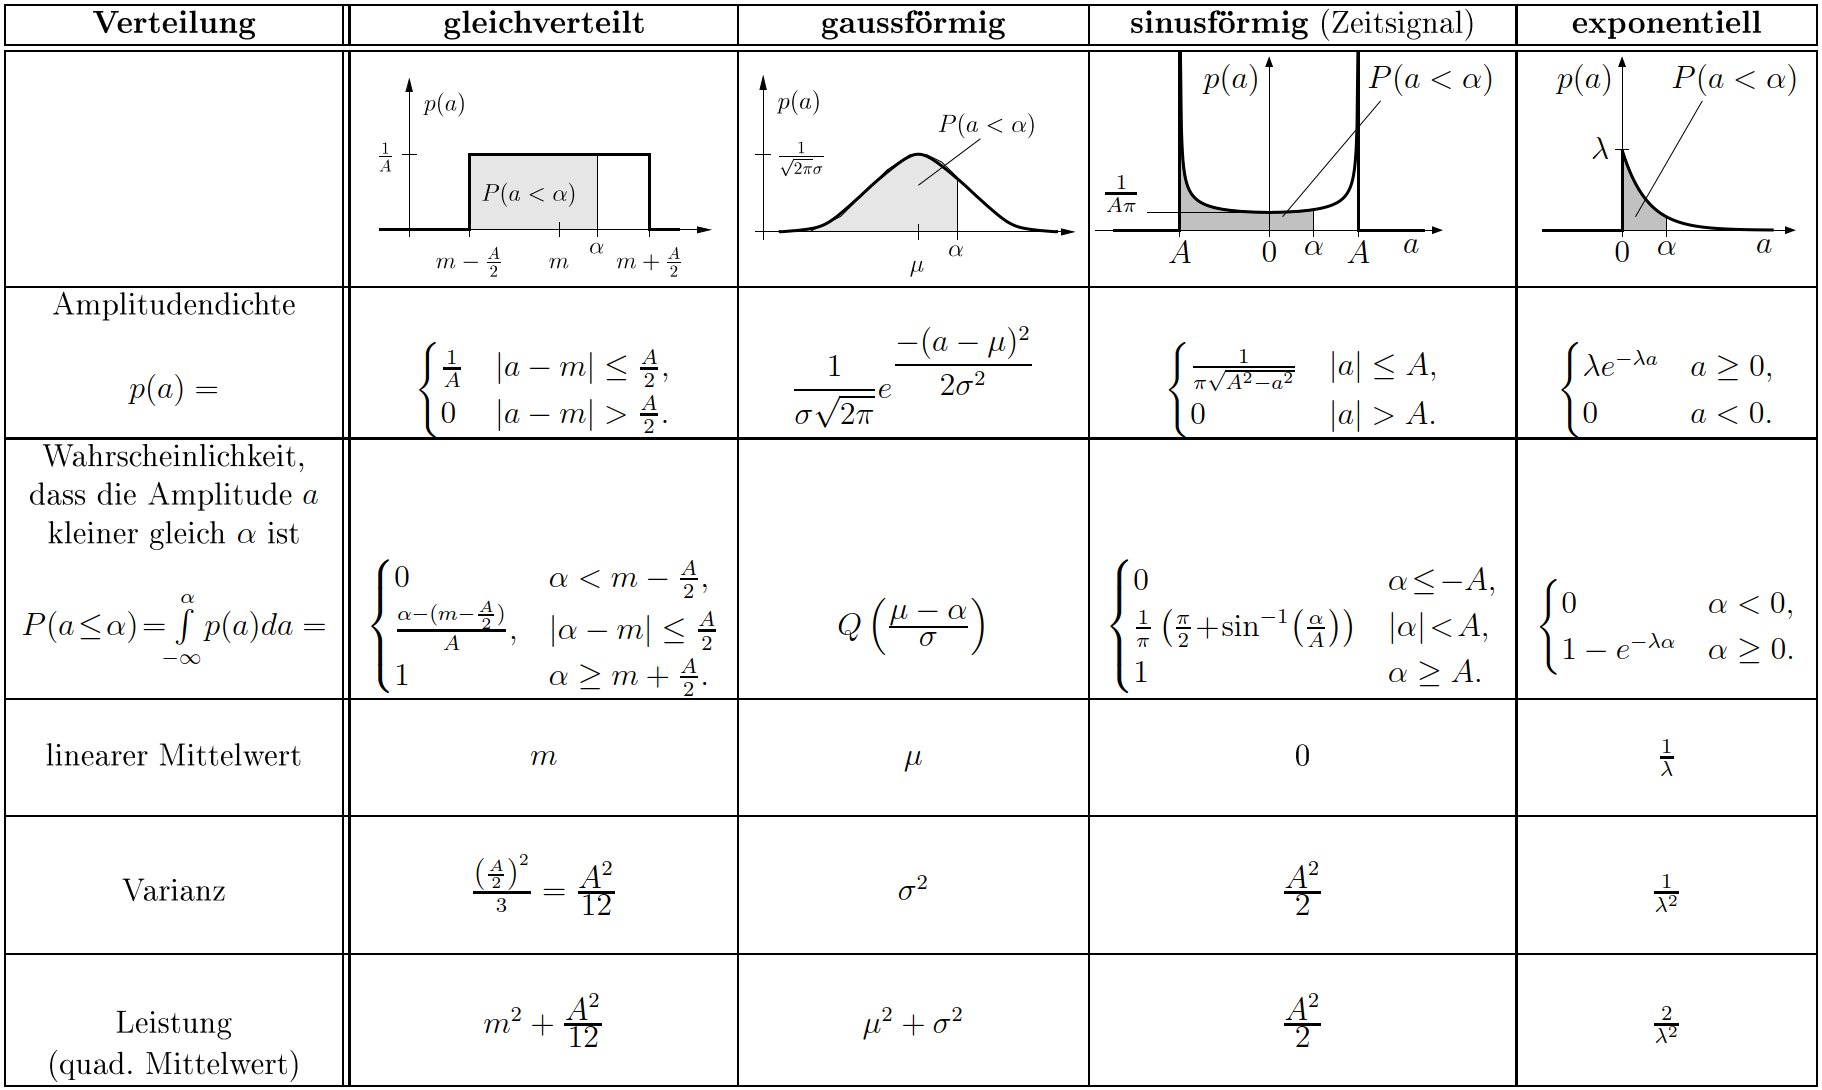
\includegraphics[width=\columnwidth]{images/zusammenstellung_dichtefunktionen.png}


\subsection{Zusammenstellung einiger Signale und ihrer Funktionen}

\resizebox{\columnwidth}{!}{
\begin{tabular}{|l||c|c|c|}
        \hline
        \multirow{2}{*}{\huge \textbf{Signal / Funktion}} & \multicolumn{2}{c|}{Endliche Signalleistung $0 < P_n < \infty, (W_n = \infty)$} & Endliche Signalenergie $W_n < \infty$ \\
        \cline{2-4}
        & periodisch ($\omega_0 = 2\pi/T_0$) & stochastisch (stationär) & abklingend, zeitbegrenzt \\
        \hline\hline
        
        Autokorrelationsfunktion (AKF) & 
        $\displaystyle \varphi(\tau) = \frac{1}{T_0} \int\limits_{-T_0/2}^{T_0/2} f(t)f(t+\tau)dt$ & 
        $\displaystyle \varphi(\tau) = \lim_{T\to\infty} \frac{1}{T} \int\limits_{-T/2}^{T/2} f(t)f(t+\tau)dt$ & 
        $\displaystyle \varphi(\tau) = \int\limits_{-\infty}^{\infty} f(t)f(t+\tau)dt$ \\
        \hline
        
        Fourier-Transformation der AKF & 
        $\displaystyle P_n = \frac{1}{T_0} \int\limits_{-T_0/2}^{T_0/2} \varphi(\tau)e^{-jn\omega_0\tau}d\tau$ & 
        $\displaystyle \Phi(j\omega) = \int\limits_{-\infty}^{\infty} \varphi(\tau)e^{-j\omega\tau}d\tau$ & 
        $\displaystyle E(j\omega) = \int\limits_{-\infty}^{\infty} \varphi(\tau)e^{-j\omega\tau}d\tau$ \\
        \hline
        
        Rücktransformation der AKF & 
        $\displaystyle \varphi(\tau) = \sum_{n=-\infty}^{\infty} P_n e^{jn\omega_0\tau}$ & 
        $\displaystyle \varphi(\tau) = \frac{1}{2\pi} \int\limits_{-\infty}^{\infty} \Phi(j\omega)e^{j\omega\tau}d\omega$ & 
        $\displaystyle \varphi(\tau) = \frac{1}{2\pi} \int\limits_{-\infty}^{\infty} E(j\omega)e^{j\omega\tau}d\omega$ \\
        \hline
        
        Amplitudenspektrum & 
        $\displaystyle c_n = \frac{1}{T_0} \int\limits_{-T_0/2}^{T_0/2} f(t)e^{-jn\omega_0 t}dt$ & 
        -- & 
        -- \\
        \hline
        
        Amplitudendichtespektrum & 
        -- & 
        -- & 
        $\displaystyle F(j\omega) = \int\limits_{-\infty}^{\infty} f(t)e^{-j\omega t}dt$ \\
        \hline
        
        Leistungsspektrum & 
        $\displaystyle P_n = |c_n|^2$ & 
        -- & 
        -- \\
        \hline
        
        Leistungsdichtespektrum & 
        -- & 
        $\displaystyle \Phi(j\omega) = E \left\{ \lim_{T \to \infty} \frac{1}{T} \left| \int\limits_{-T/2}^{T/2} f(t)e^{-j\omega t}dt \right|^2 \right\}$ & 
        -- \\
        \hline
        
        Energiedichtespektrum & 
        -- & 
        -- & 
        $\displaystyle E(j\omega) = |F(j\omega)|^2$ \\
        \hline
        
        Energie & 
        -- & 
        -- & 
        $\displaystyle W = \varphi(0) = \frac{1}{2\pi} \int\limits_{-\infty}^{\infty} E(j\omega)d\omega$ \\
        \hline
        
        Leistung & 
        $\displaystyle P = \varphi(0) = \sum_{n=-\infty}^{\infty} P_n$ & 
        $\displaystyle P = \varphi(0) = \frac{1}{2\pi} \int\limits_{-\infty}^{\infty} \Phi(j\omega)d\omega$ & 
        -- \\
        \hline
        
        Fourier-Reihe & 
        $\displaystyle f(t) = \sum_{n=-\infty}^{\infty} c_n e^{jn\omega_0 t}$ & 
        -- & 
        -- \\
        \hline
        
        Fourier-Integral & 
        -- & 
        -- & 
        $\displaystyle f(t) = \frac{1}{2\pi} \int\limits_{-\infty}^{\infty} F(j\omega)e^{j\omega t}d\omega$ \\
        \hline
    \end{tabular}}

\subsection{Beispiele -- Amplitudendichten}
\label{Beispiele - Amplitudendichte}

\subsubsection{Sinus}

\begin{minipage}[c]{0.48\columnwidth}
    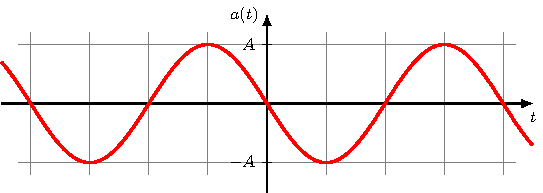
\includegraphics[width=\columnwidth]{images/PDF/sinussignal.pdf} 
\end{minipage}
\hfill
\begin{minipage}[c]{0.48\columnwidth}
    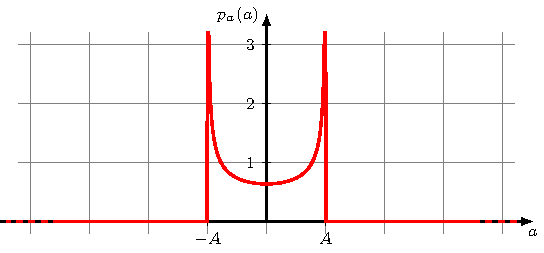
\includegraphics[width=\columnwidth]{images/PDF/sinussignal_amplitudendichte.pdf} 
\end{minipage}


\subsubsection{Dreieck}

\begin{minipage}[c]{0.48\columnwidth}
    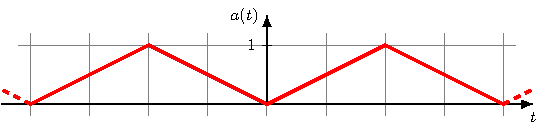
\includegraphics[width=\columnwidth]{images/PDF/dreiecksignal.pdf} 
\end{minipage}
\hfill
\begin{minipage}[c]{0.48\columnwidth}
    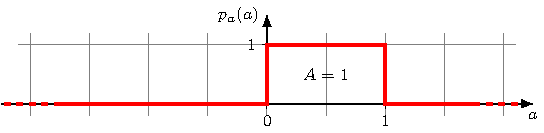
\includegraphics[width=\columnwidth]{images/PDF/dreiecksignal_amplitudendichte.pdf} 
\end{minipage}


\subsubsection{Rechteck}
\label{Rechteck} 

\begin{minipage}[c]{0.48\columnwidth}
    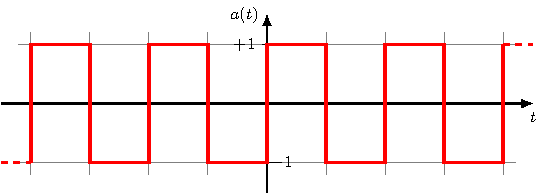
\includegraphics[width=\columnwidth]{images/PDF/rechtecksignal.pdf} 
\end{minipage}
\hfill
\begin{minipage}[c]{0.48\columnwidth}
    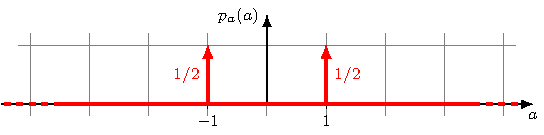
\includegraphics[width=\columnwidth]{images/PDF/rechtecksignal_amplitudendichte.pdf} 
\end{minipage}

